\documentclass[12pt]{article}

\usepackage{graphicx}
\graphicspath{ {./} }
\usepackage{paralist}
\usepackage{amsfonts}
\usepackage{amsmath}
\usepackage{hhline}
\usepackage{booktabs}
\usepackage{multirow}
\usepackage{multicol}
\usepackage{url}
\usepackage{hyperref}

\oddsidemargin -10mm
\evensidemargin -10mm
\textwidth 160mm
\textheight 200mm
\renewcommand\baselinestretch{1.0}

\pagestyle {plain}
\pagenumbering{arabic}

\newcounter{stepnum}

%% Comments

\usepackage{color}

\newif\ifcomments\commentstrue

\ifcomments
\newcommand{\authornote}[3]{\textcolor{#1}{[#3 ---#2]}}
\newcommand{\todo}[1]{\textcolor{red}{[TODO: #1]}}
\else
\newcommand{\authornote}[3]{}
\newcommand{\todo}[1]{}
\fi

\newcommand{\wss}[1]{\authornote{blue}{SS}{#1}}

\title{Assignment 4, Design Specification}
\author{SFWRENG 2AA4}

\begin{document}

\maketitle
This Module Interface Specification (MIS) document contains modules, types and
methods for implementing the game \textbf{2048}. At the start of each game, the user is provided with a Board of 4x4 tiles with any two random tiles with value 2 (90\%) or 4 (10\%), whereas all other tiles are initialized with a value of 0.
The user can choose to make their move by typing ”w , a, s, d”, where `w' is for moving and merging the tiles in upward direction, `a' for left, `s' for down and `d' for right. This will change the state of the Board and shift the tiles with non zero values towards the input direction. The Tiles with the same value merge
into one when they touch and increase the total score of the user. Add them up to reach 2048! After every move that is feasible, one random tile with 0
value takes up the value of 2 or 4.
Finally, the game can be launched and play by typing \texttt{make demo} in terminal.

\begin{center}
 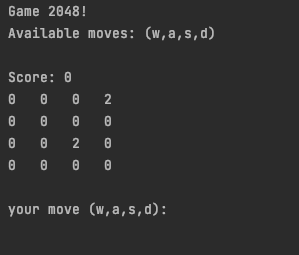
\includegraphics[width=0.4\textwidth]{terminal-1.png}
 \hspace{1.4cm}
 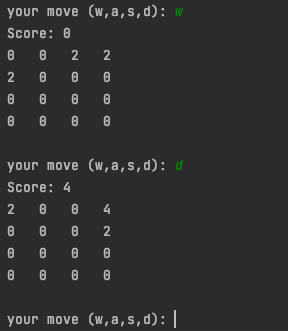
\includegraphics[width=0.4\textwidth]{terminal-2.png}\\
  \hspace{1.6cm}
  Initial state of game
  \hspace{1.9cm}
  Score update when two tiles with value 2 merge
\end{center}

\newpage

\section{Overview of the design}

This design applies Module View Specification (MVC) design pattern and Singleton design pattern. The MVC components
are \textit{Board} (model module), and \textit{Game} (View and Controller module).
Singleton pattern is specified and implemented for \textit{Game}.

\medskip
The MVC design pattern is specified and implemented in the following way: the module \textit{Board} stores the state of the game board and the score of the user. A view module \textit{Game} can display the state of the game board and game using a text-based graphics. \textit{Game} is also responsible for handling input actions. For \textit{Game}, use the main() method to run the game.

\vspace{5cm}

\subsection*{Likely Changes my design considers:}

\begin{itemize}
  \item Data structure used for user login to keep track of their highest score.
  \item The visual representation of the game such as UI layout.
  \item Change in game ending conditions to adjust the difficulty of the game.
  \item Modularization could be done with more precision.
  \item Implementing GUI to make it more interactive.
\end{itemize}

\newpage

\section* {MoveT Module}

\subsection*{Module}

MoveT

\subsection* {Uses}

N/A

\subsection* {Syntax}

\subsubsection* {Exported Constants}

None

\subsubsection* {Exported Types}

MoveT = \{w, a, s, d\}

\medskip

\noindent \textit{//w is for merging in upper direction , a for left direction,\\
 			s for downward direction, d for right direction}

\subsubsection* {Exported Access Programs}

None

\subsection* {Semantics}

\subsubsection* {State Variables}

None

\subsubsection* {State Invariant}

None

\newpage

\section* {Tile Module}

\subsection* {Template Module}

Tile

\subsection*{Uses}

None

\subsection* {Syntax}

\subsection*{Exported Constants}

None

\subsection*{Exported Types}

None

\subsubsection* {Exported Access Programs}

\begin{tabular}{| l | l | l | p{6cm} |}
\hline
\textbf{Routine name} & \textbf{In} & \textbf{Out} & \textbf{Exceptions}\\
\hline
Tile & ~ & Tile & \\
\hline
Tile & $\mathbb{Z}$ & Tile & IllegalArgumentException\\
\hline
getValue & & $\mathbb{Z}$ & \\
\hline
setValue & $\mathbb{Z}$ &  & IllegalArgumentException\\
\hline
toString &  & String & \\
\hline
\end{tabular}

\subsection* {Semantics}

\subsection*{State Variables}

value: $\mathbb{Z}$

\subsection*{State Invariant}

None

\subsection*{Assumptions}

None

\subsubsection* {Access Routine Semantics}

new Tile():

\begin{itemize}
  \item output: out $:=$ self
  \item transition: this.value = 0
  \item exception: None
\end{itemize}

\noindent new Tile(number):

\begin{itemize}
  \item output: out $:=$ self
  \item transition: this.value = number
  \item exception: IllegalArgumentException
\end{itemize}

\noindent getValue():

\begin{itemize}
  \item output: out $:=$ this.value
  \item exception: None
\end{itemize}

\noindent setValue(value):
\begin{itemize}
  \item transition: this.value $:=$ value
  \item exception: IllegalArgumentException
\end{itemize}

\noindent toString():
\begin{itemize}
  \item out: out $:=$ String.valueOf(value)
  \item exception: None
\end{itemize}

\newpage
\section* {Board ADT Module}

\subsection*{Template Module}

Board

\subsection* {Uses}

Tile

\subsection* {Syntax}

\subsubsection* {Exported Types}

None

\subsubsection* {Exported Constant}

None

\subsubsection* {Exported Access Programs}

\begin{tabular}{| l | l | l | l |}
\hline
\textbf{Routine name} & \textbf{In} & \textbf{Out} & \textbf{Exceptions}\\
\hline
Board & ~ & Board & \\
\hline
Board & seq of (seq of Tile) & Board & \\
\hline
Board & $\mathbb{Z}$ & Board & \\
\hline
getScore & ~ & $\mathbb{Z}$ & \\
\hline
highestTile & ~ & $\mathbb{Z}$ & \\
\hline
spawnRandom & ~ & ~ & \\
\hline
move & MoveT & ~ & IllegalArgumentException\\
\hline
gameWon & ~ & $\mathbb{B}$ & \\
\hline
gameOver & ~ & $\mathbb{B}$ & \\
\hline
up & ~ & ~ & \\
\hline
down & ~ & ~ & \\
\hline
vMerge & ~ & ~ & \\
\hline
left & ~ & ~ & \\
\hline
right & ~ & ~ & \\
\hline
hMerge & ~ & ~ & \\
\hline
toString & ~ & String & \\
\hline

\end{tabular}

\subsection* {Semantics}

\subsubsection* {State Variables}

board: Sequence of (Sequence of Tile) \\
edge: $\mathbb{Z}$ \\
score: $\mathbb{Z}$

\subsubsection* {State Invariant}

None

\subsubsection* {Assumptions}

\begin{itemize}
  \item The constructor Board is called for each object instance before any other access routine
  is called for that object.
  \item SpawnRandom needs to be called independently two time swhen initiating the game.
  \item Methods will be used wisely to control the flow of the game.
\end{itemize}

\subsubsection* {Access Routine Semantics}

new Board():
\begin{itemize}
\item transition: $\forall$(i : Integer $|$ i $<$ 4 $\Rightarrow$ ($\forall$(j : Integer $|$ j $<$ 4 $\Rightarrow$ board[i][j] $:=$ new Tile())))
\item output: $out := \mathit{self}$
\item exception: None
\end{itemize}

\noindent new Board($tt$):
\begin{itemize}
\item transition: $\forall$ (i: Integer $|$ i $<$ 4 $\Rightarrow$ board[i] $:=$ tt[i])
\item output: $out := \mathit{self}$
\item exception: None
\end{itemize}

\noindent new Board(factor):
\begin{itemize}
\item transition: $\forall$(i : Integer $|$ i $<$ 4 $\Rightarrow$ ($\forall$(j : Integer $|$ j $<$ 4 $\Rightarrow$ board[i][j] $:=$ new Tile(( $factor + i + j + 1) * ( i + j + 1)$)))))
\item output: $out := \mathit{self}$
\item exception: None
\end{itemize}

\noindent getScore():
\begin{itemize}
\item transition: none
\item output: $out :=$ this.score
\item exception: None
\end{itemize}

\noindent highestTile():
\begin{itemize}
\item transition: none
\item output: $out :=$ high, where\\
$\forall$(i : Integer $|$ i $<$ 4 $\Rightarrow$ ($\forall$(j : Integer $|$ j $<$ 4 $\Rightarrow$ (board[i][j].getValue() $>$ high $\Rightarrow$ high $:=$ board[i][j].getValue()))))
\item exception: None
\end{itemize}

\noindent spawnRandom():
\begin{itemize}
\item output: $out :=$ board[$y$][7 - $x$]
\item exception: $exc :=$ ($\neg$ validateCell($x, y) \Rightarrow$ IndexOutOfBoundsException)
\end{itemize}

\noindent move(direction):
\begin{itemize}
\item transition: (direction == MoveT.w $\Rightarrow$  up() $|$ (direction == MoveT.a $\Rightarrow$  left() $|$ (direction == MoveT.s $\Rightarrow$  down() $|$ (direction == MoveT.d $\Rightarrow$  right() $|$ IllegalArgumentException))))
\item output: None
\item exception: IllegalArgumentException
\end{itemize}

\noindent gameWon():
\begin{itemize}
  \item transition: None
  \item output: out := (highestTile() == 2048 $\Rightarrow$ true $|$ false)
  \item exception: None
\end{itemize}

\noindent gameOver():
\begin{itemize}
  \item transition: None
  \item output: out := (count == 16 $\Rightarrow$ true $|$ false), where\\
  count is the number of tiles which can't be combined with it's adjacent tiles.
  \item exception: None
\end{itemize}

\noindent up():
\begin{itemize}
  \item transition: $\forall$(i : Integer $|$ i $<$ 4 $\Rightarrow$ ($\forall$(j: Integer $|$ j $<$ 4 $\Rightarrow$ (board[j][i].getValue() != 0 $\Rightarrow$ (edge $<=$ j $\Rightarrow$ vMerge(j, i, "up"))))))
  \item output: None
  \item exception: None
\end{itemize}

\noindent down():
\begin{itemize}
  \item transition: $\forall$(i : Integer $|$ i $<$ 4 $\Rightarrow$ ($\forall$(j = 3 : Integer $|$ j $>= 0$ $\Rightarrow$ (board[j][i].getValue() != 0 $\Rightarrow$ (edge $>=$ j $\Rightarrow$ vMerge(j, i, "down"))))))
  \item output: None
  \item exception: None
\end{itemize}

\noindent vMerge():
\begin{itemize}
  \item transition: score is updated as any two tile merges in vertical direction
  \item output: None
  \item exception: None
\end{itemize}

\noindent left():
\begin{itemize}
  \item transition: $\forall$(i : Integer $|$ i $<$ 4 $\Rightarrow$ ($\forall$(j: Integer $|$ j $<$ 4 $\Rightarrow$ (board[i][j].getValue() != 0 $\Rightarrow$ (edge $<=$ j $\Rightarrow$ hMerge(i, j, "left"))))))
  \item output: None
  \item exception: None
\end{itemize}

\noindent right():
\begin{itemize}
  \item transition: $\forall$(i : Integer $|$ i $<$ 4 $\Rightarrow$ ($\forall$(j = 3 : Integer $|$ j $>= 0$ $\Rightarrow$ (board[i][j].getValue() != 0 $\Rightarrow$ (edge $>=$ j $\Rightarrow$ hMerge(i, j, "right"))))))
  \item output: None
  \item exception: None
\end{itemize}

\noindent hMerge():
\begin{itemize}
  \item transition: score is updated as any two tile merges in horizontal direction
  \item output: None
  \item exception: None
\end{itemize}

\noindent toString():
\begin{itemize}
  \item transition: None
  \item output: out $:=$ s, where\\
  $\forall$(i : Integer $|$ i $<$ 4 $\Rightarrow$ ($\forall$(j: Integer $|$ j $<$ 4 $\Rightarrow$ (s += board[i][j].toString() + "   "))))
  \item exception: None
\end{itemize}

\newpage


\section*{Critique of Design}

\begin{itemize}
  \item I've specified Board module as ADT over abstract object, because It is more convenient to create a new instance of the board after the user choose to restart a game.
  \item All the methods added have high usability for the view module to display the status of the game. Therefore, the design pattern used is highly essential.
  \item The $move$ method in $Board$ preserves the principle of minimality as it combines the use of up, down, left and right methods. I design this module in this way is to ensure there is no delay or friction with the model module since the same method could serve the purpose of having 4 different methods.
  \item The three constructors in Board improve the flexibilty of the module. The user can choose to play with a board initialized with randomly generated dots or a board that is customized or pre-defined. Also, from a testing perspective, methods can be easily tested if the board is pre-defined compared to a randomly generated board.
  \item The test cases are designed to validate the correctness of the program based on the requirement and reveal errors or unusual behavior during program execution, every access routine has at least one test case. One exception is made for $spawnRandom$ method in Board because the $spawnRandom$ method adds a random Tile to the board, there are no efficient ways to test the correctness of adding a randomly generated Tile.
  \item In $Board$, the result of $up$, $down$, $left$ and $right$ were tested using the total score generated from the merges in that move.
  \item Did not build any test cases for testing the controller module since the implementation of the controller's access methods uses methods from the model and view. The test cases for the model are in $TestBoard.java$
  \item The use of MVC also keeps my design safe and reduces the chance of transition. MVC decomposes into three separate components where the model component encapsulates the game's internal data and status, where the view shows the game status, and where the controller deals with the input behaviour to execute the relevant measures to react to the events.
  \item I architecture with the application of MVC achieve high cohesion and low coupling. The MVC maintains strong cohesion since within - module it groups similar features. The architecture is also low because of its mostly separate modules (model, display, controller). A improvement in one of the modules thus has little significant influence on the other.
  \item I've found it easier to use Singleton designs than to use abstract object static approaches. During the development process certain alerts about the method or variables need to be accessed statically for the application of static methods and variables. For the singleton model, all these challenges are eliminated and a simpler development is achieved.

\end{itemize}
\vspace{3cm}
\section*{Answers to Questions:}

Q1: Draw a UML diagram for the modules in A3.

\medskip
\medskip

\noindent Q2: Draw a control flow graph for convex hull algorithm.

\begin{center}
  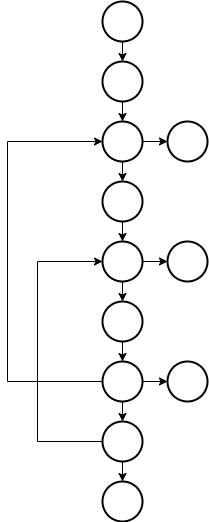
\includegraphics[width=0.4\textwidth]{Control.png} \\
  \vspace{2cm}
  The control flow graph is constructed using https://app.diagrams.net/
\end{center}

\end {document}